\documentclass[compsoc]{IEEEtran}
\usepackage{graphicx}
\usepackage{amsmath}
\usepackage{authblk}
\usepackage[english]{babel}
\usepackage{blindtext}
%\usepackage[ruled,vlined,linesnumbered]{algorithm2e}
%\usepackage{algorithmic,float}
\usepackage{setspace}
\usepackage{amsfonts}
\usepackage{hyperref}
\graphicspath{ {./images/} }
\usepackage{subfig}
\usepackage{fontspec}
\usepackage{listings}
\usepackage{amsmath}
\usepackage{mathabx}
\usepackage[bottom]{footmisc}
\newfontfamily\listingsfont[Scale=.7]{inconsolata}\usepackage[font=footnotesize,labelfont=bf]{caption}
%\captionsetup[algorithm2e]{font=footnotesize}
\usepackage[table,xcdraw]{xcolor}
\usepackage[utf8]{inputenc}
\title{Assignment: Checkerboard classification problem}
\author{David Bertoldi -- 735213 \\ email: d.bertoldi@campus.unimib.it}
\affil{Department of Informatics, Systems and Communication}
\affil{University of Milano-Bicocca}
\date{October 2022}


\begin{document}

\maketitle 



\section{Inspecting the data}
The data provided consists of a set of points $X \in \{(x_1, x_2) \ | \ 10 \leq x_1 \leq 20 \wedge 10 \leq x_2 \leq 20 \}$ and a set of binary labels $y \in \{0, 1\}$.
The points in $X$ follow a uniform distribution with mean $\mu = 14.97$ and variance $\sigma = 8.3$; the $0$s and $1$s in $y$ are quite uniformely distributed with 
a mean of $\mu = 0.498$. That means the 2 classes are balanced. \par
If we map each $i^{th}$ point of $X$ with the $i^{th}$ element of $y$ and assign for each different element of $y$ a different color we get a \emph{check pattern} over the points of $X$, partitioning the 4000 points in 6 columns and 6 rows.
The result can be observed in Figure \ref{fig:checkerboard}

\begin{figure}[ht!]
\centering                                                                        
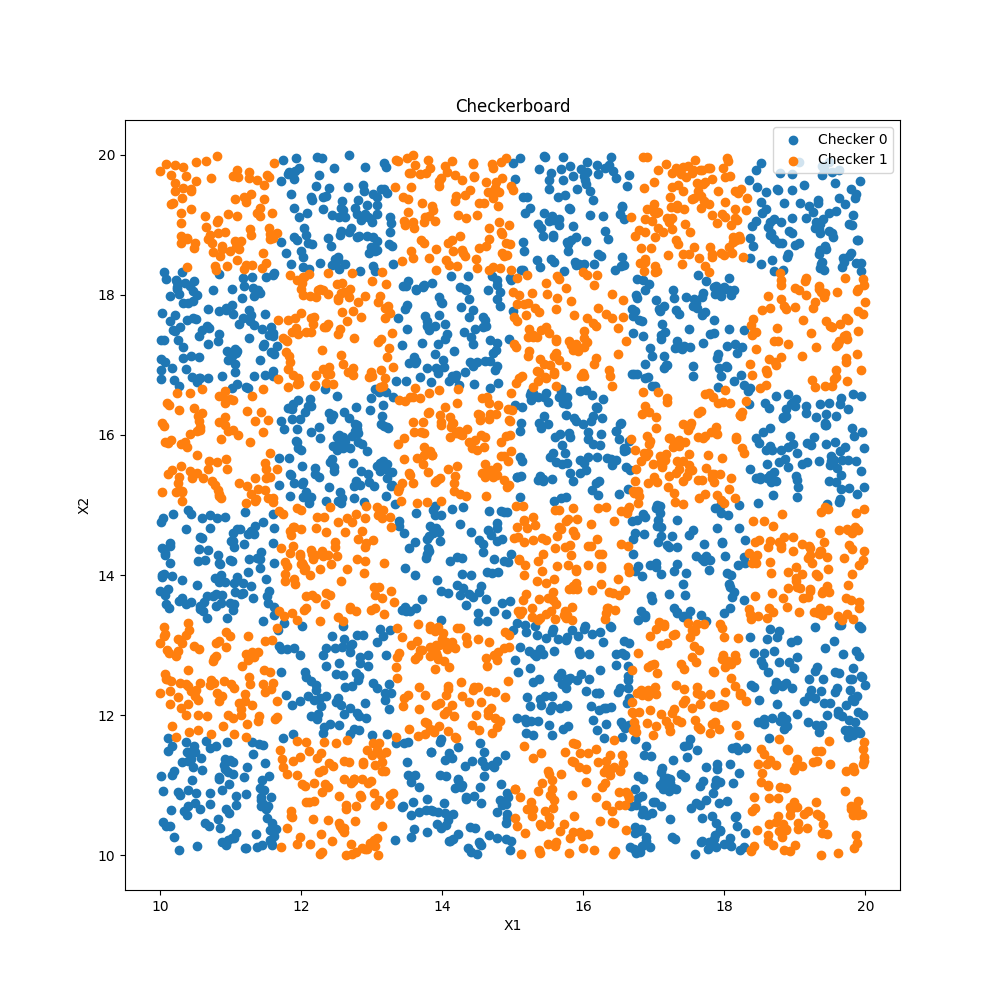
\includegraphics[width=3.5in]{../images/checkerboard.png}
\captionsetup{justification=centering}                                                                                                                                   
\caption{Visualization of the dataset}
\label{fig:checkerboard}                                                                                                                                                           
\end{figure}

\section{Preparing the data}
Before using the data we want to standardize features by removing the mean and scaling to unit variance. Standardization of a dataset is a common requirement for many machine learning estimators: they might behave badly if the individual features are not standard normally distributed. That's why we want to remove the mean $\mu$ and scale $\sigma$ to unit variance. \par
In order to do so, we use the \texttt{StandardScaler} from \texttt{sklearn.preprocessing} package. After this operation we have  $\mu=1.4 \cdot 10^{-9}$ (very close to 0) and $\sigma = 1$, which is exactly what we wanted.

\section{Building the network and training}
\subsection{Data split}
The dataset does not provide a set of points to be used for validation and testing. So we split the dataset into three partitions: 72\% of points are used for the training, 15\% for validation and 13\% for testing. Having less points used for training had proved to perform worse.

\subsection{Network}
The network chosen is a Feed-Forward Neural Network with non-linear activation functions. We tried two approaches: \texttt{tanh} and \texttt{LeakyReLU}. The first one seemed to be the right choice because it is possible to emulate the \emph{check pattern} with the following formula:
\[sin(y) \leq cos(x)\]
and since the definition of $tanh(x)$ can be derived from $cos(ix)$ and $sin(ix)$, there could had been some facilitation on using such activator. Unfortunately, despite the good results,
\texttt{LeakyReLU} performed better and for this reason we used it as a definitive one. \par

Because we are trying to classify points between two classes, the output function is a sigmoid. \par

Finally, the network architecture is composed by 4 hidden dense layers of rispectively 200, 150, 100 and 50 nodes. We tried with less hidden layers (2 and 3) and less nodes for each
layer (100, 50, 25, 10) but the performance where worse in terms of convergence speed and decision boundaries: 
with the same amount of epochs we had a drop of $5\%$ to $10\%$ in accuracy on the validation set (also in accordance with the evolution of decision boundaries).
Since the different configurations had similar training times, we chose this configuration over a lighter one generating a negligible difference in overfitting. \par

Each node uses \texttt{LeakyReLU} as activator function with $\alpha=0.1$. The output node computes the sigmoid logistic function so that the output ranges between $0$ and $1$.

\begin{figure}[ht!]
\centering                                                                        
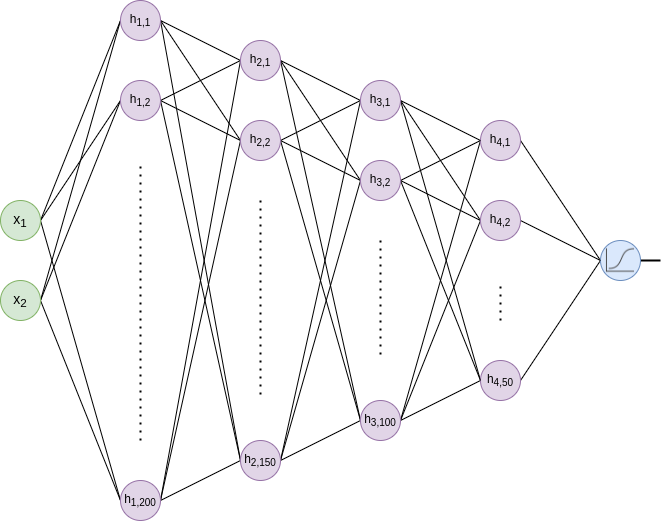
\includegraphics[width=3.5in]{../images/nn-1.png}
\captionsetup{justification=centering}                                                                                                                                   
\caption{The neural network with 4 dense hidden layers}
\label{fig:nn}                                                                                                                                                           
\end{figure}

\subsection{Training}
The choice of the optimizer was among \emph{SGD}, \emph{RMSProp} and \emph{Adam}. We tried all of them and chose \emph{Adam} 
with learning rate of $0.001$, $\beta_{1}=0.9$ and $\beta_{2}=0.999$ because it seemed to escape better from local minima, converging faster and giving better accuracy. \par
Because we are treating a binary classification problem, we used the \emph{binary crossentropy} loss function.
Figure \ref{fig:decision} shows how the decision boundaries evolve over the test dataset every 10 epochs.

\begin{figure}[ht!]
\begin{tabular}{cccc}
\subfloat[1 epoch]{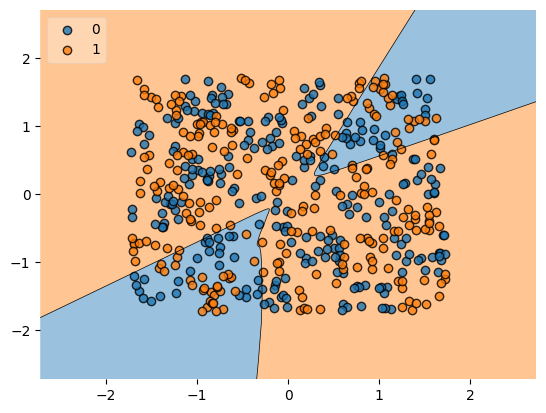
\includegraphics[width = 1in]{../images/regions/0-region.png}} &
\subfloat[10 epochs]{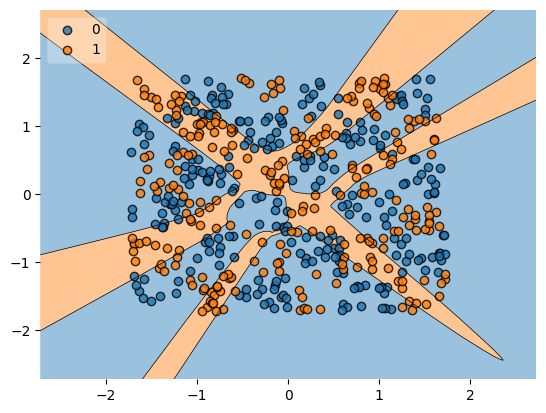
\includegraphics[width = 1in]{../images/regions/10-region.png}} &
\subfloat[20 epochs]{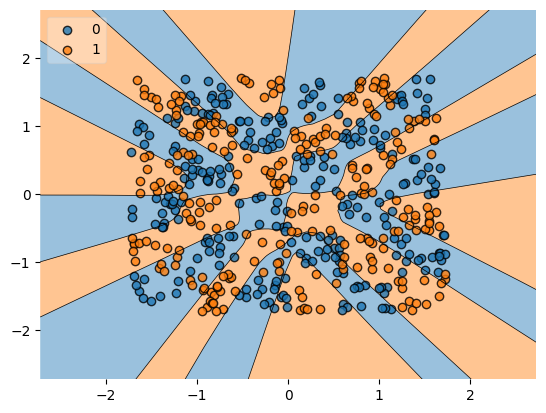
\includegraphics[width = 1in]{../images/regions/20-region.png}}\\
\subfloat[30 epochs]{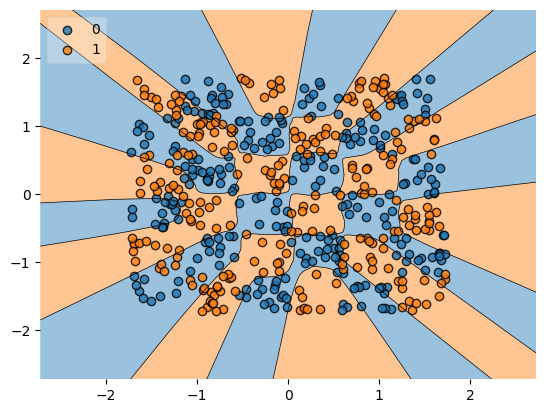
\includegraphics[width = 1in]{../images/regions/30-region.png}} &
\subfloat[40 epochs]{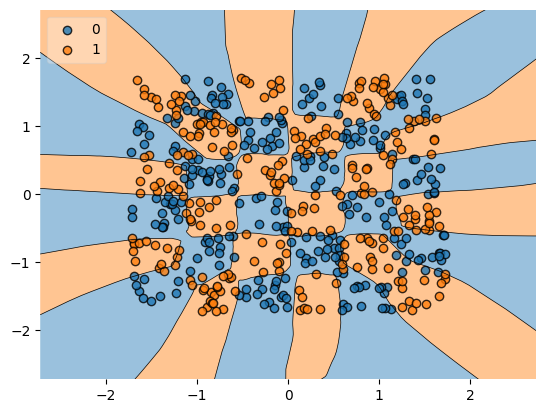
\includegraphics[width = 1in]{../images/regions/40-region.png}} &
\subfloat[50 epochs]{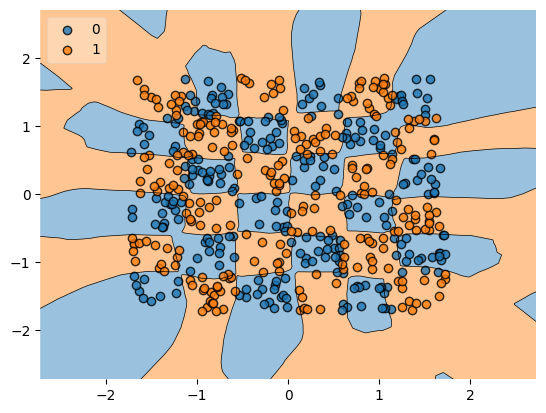
\includegraphics[width = 1in]{../images/regions/50-region.png}}\\
\subfloat[60 epochs]{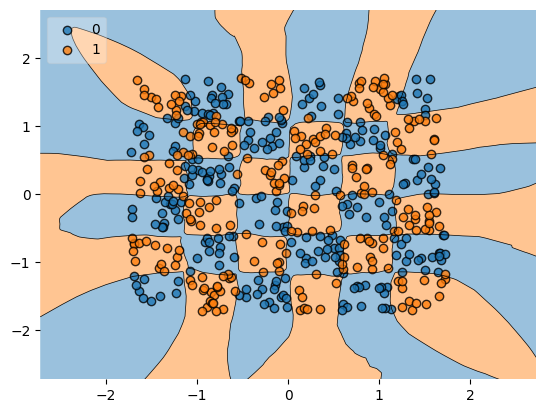
\includegraphics[width = 1in]{../images/regions/60-region.png}} &
\subfloat[70 epochs]{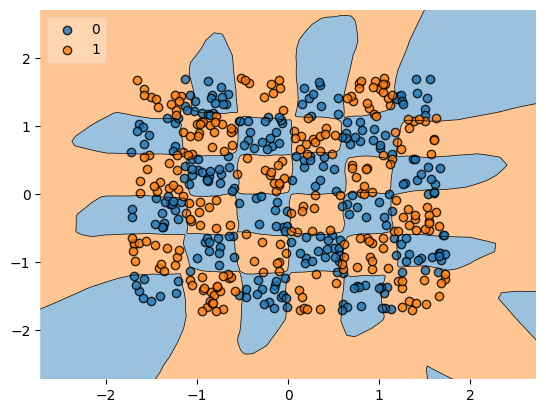
\includegraphics[width = 1in]{../images/regions/70-region.png}} &
\subfloat[80 epochs]{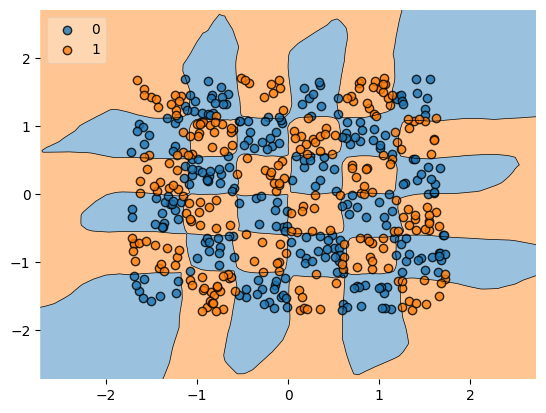
\includegraphics[width = 1in]{../images/regions/80-region.png}} 
\end{tabular}
\caption{Evolution of decision boundaries during the training}
\label{fig:decision}                                                                                                                                                           
\end{figure}

Talking about the batch size, we tried with 16 and 8 samples at time and from with minibatches of 4 to 1 samples, achieving an optimal performance with a batch of 4 elements. \par
 
Figure \ref{fig:loss} and Figure \ref{fig:acc} plots the trend of the loss function and its accuracy over the validation set. The first one measures the score that penalizes the probabilities based on the distance from the expected value. \par
The second one represents the ratio between the number of correct predictions to the total number of predictions; this metric is preferable over the precision because accuracy treats
all classes with the same importance while precision measures the model's accuracy only in classifying a sample as positive.

\begin{figure}[ht!]
\centering                                                                        
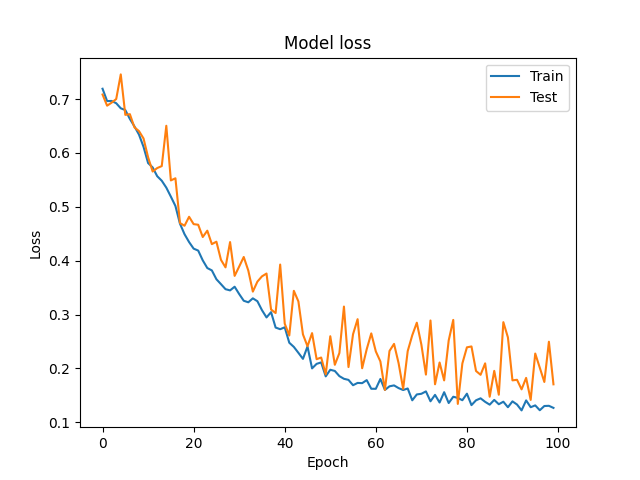
\includegraphics[width=3.5in]{../images/loss-4000-6-binary_crossentropy-adam-100-4.png}
\captionsetup{justification=centering}                                                                                                                                   
\caption{Loss}
\label{fig:loss}                                                                                                                                                           
\end{figure}


\begin{figure}[ht!]
\centering                                                                        
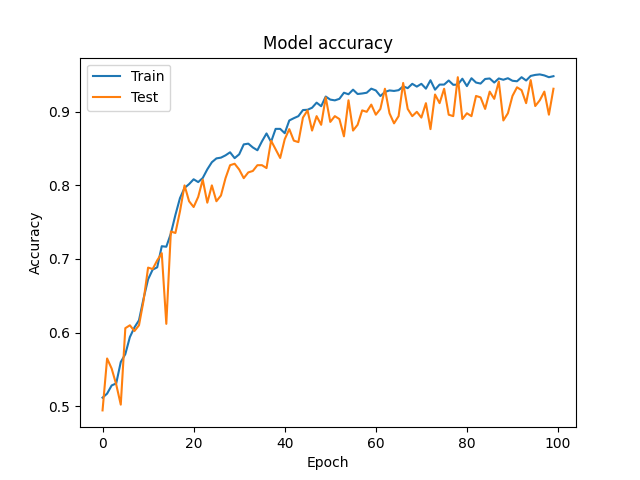
\includegraphics[width=3.5in]{../images/accuracy-4000-6-binary_crossentropy-adam-100-4.png}
\captionsetup{justification=centering}                                                                                                                                   
\caption{Accuracy}
\label{fig:acc}                                                                                                                                                           
\end{figure}



\section{Analysis}
From Figures \ref{fig:decision}, \ref{fig:loss} and \ref{fig:acc} we saw that the model correctly classifies almost all the points after 60 epochs (accuracy $\geq 90\%$ both on training and validation). This is a good result but we expected that the model could figure out what is the general rule under the provided classification.  
As we can see from Figure \ref{fig:decision}, as the accuracy of the model increases, it is clear that the model fails to recognize the \emph{check pattern} itself. Even if it is true that the accuracy reaches a score of $94\%$ during validation, the model overfits the data and could not generalize the pattern beyond the region occupied by the training data. 
This means that a point outside the original training set (\emph{e.g.} $(9, 19)$) is classified by the model in the same way as the nearest square (\emph{e.g.} orange instead of blue, even if the checker on its left is orange). \par
What happens is that the pattern predicted by the model is a checkerboard with the external checkers stretched infinitely outwards.
Figure \ref{fig:trend} shows a simplified trend in model's prediction if we increase the number of epochs.

\begin{figure}[ht!]
\centering                                                                        
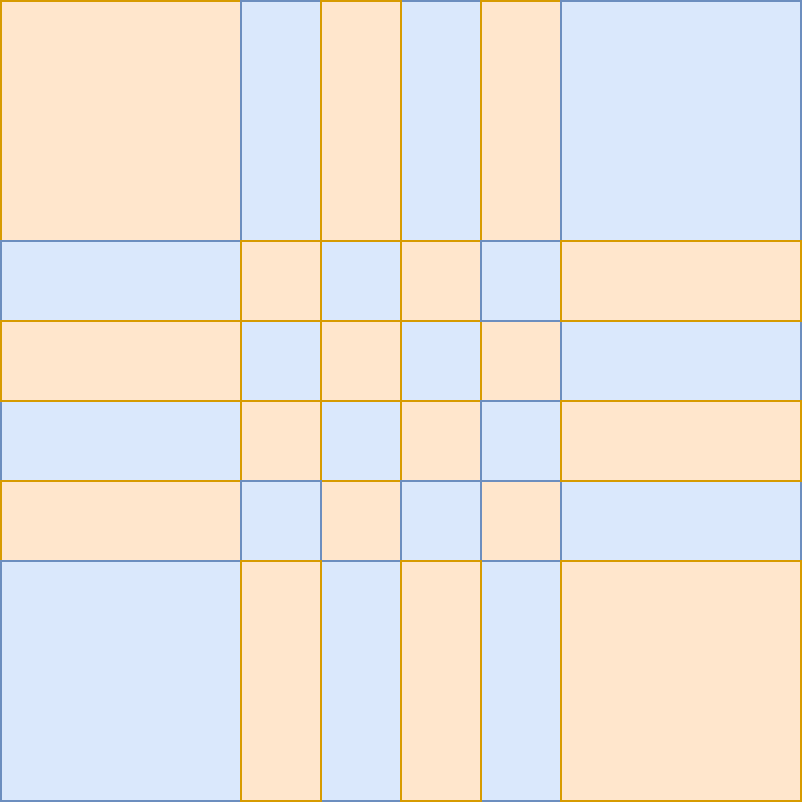
\includegraphics[width=2.5in]{../images/trend.png}
\captionsetup{justification=centering}                                                                                                                                   
\caption{Trend of the decision boundaries of the model}
\label{fig:trend}                                                                                                                                                         
\end{figure}

This result is in line with the behaviour of a similar problem: a Feedforward Network fails to learn the missing colors of a checkerboard with missing squares and the more it learns from training data, the worse it does on test data\cite{unlearnable}. \par

\section{Validation}
After the analysis we validated the model with the test dataset and calculate the confusion matrix in order to visualize the performance of the model's predictrion.
\begin{figure}[ht!]
\centering                                                                        
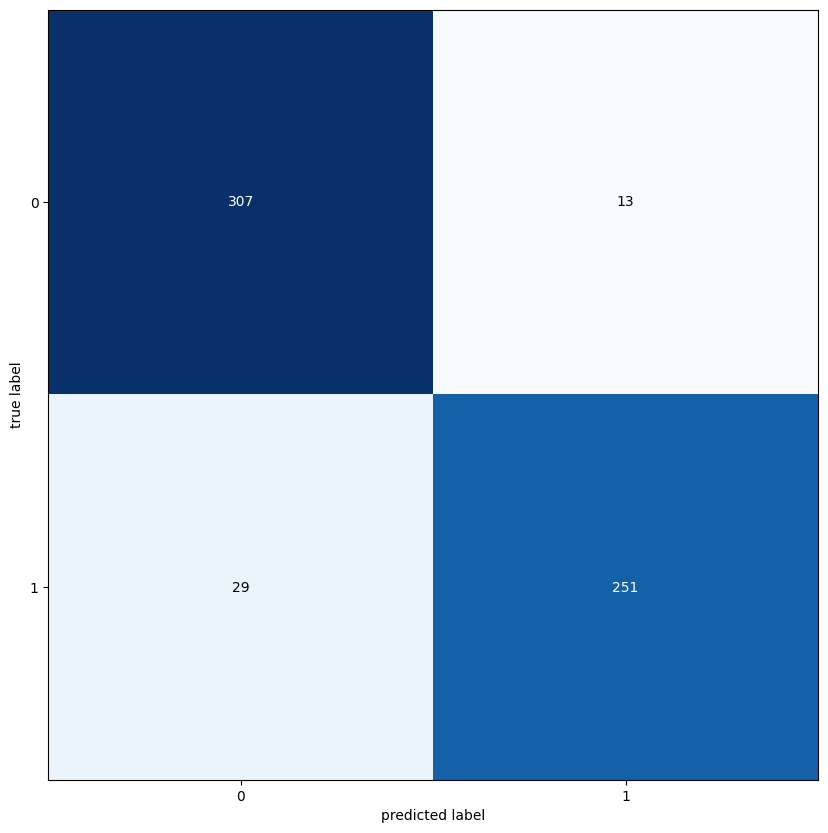
\includegraphics[width=2.5in]{../images/cm.png}
\captionsetup{justification=centering}                                                                                                                                   
\caption{Confusion matrix calculated on the test dataset}
\label{fig:cm}
\end{figure}
From Figure \ref{fig:cm} we had the cofirmation that the accuracy of the model stayed above the $93\%$. We had another confirmation from
the decision boundaries of the model in its maximum accuracy state (Figure \ref{fig:regiontest}).

\begin{figure}[ht!]
\centering                                                                        
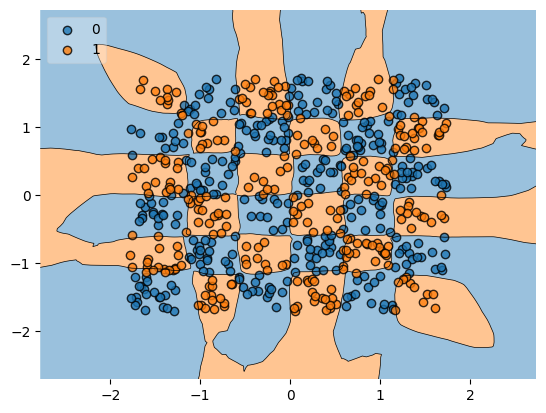
\includegraphics[width=3in]{../images/region.png}
\captionsetup{justification=centering}                                                                                                                                   
\caption{Decision boundaries over the test dataset}
\label{fig:regiontest}
\end{figure}



\section{Alternative problem}
The following problem is a variation of the previously presentend one. What is changing is the number of samples (from 4000 to 1000) and the number of checkers (from 36 to 400). This means that the frequency of samples is much more rare while leaving almost unchanged means and variation ($\mu=15.09$, $\sigma=8.64$). \par
Figure \ref{fig:checkerboard2} shows the new problem and demonstrates that it is impossible for the human brain to recognize the \emph{checker pattern}. The checkers are too thin and frequent and the data is not enough in order to recognize any pattern. \par
\begin{figure}[ht!]
\centering                                                                        
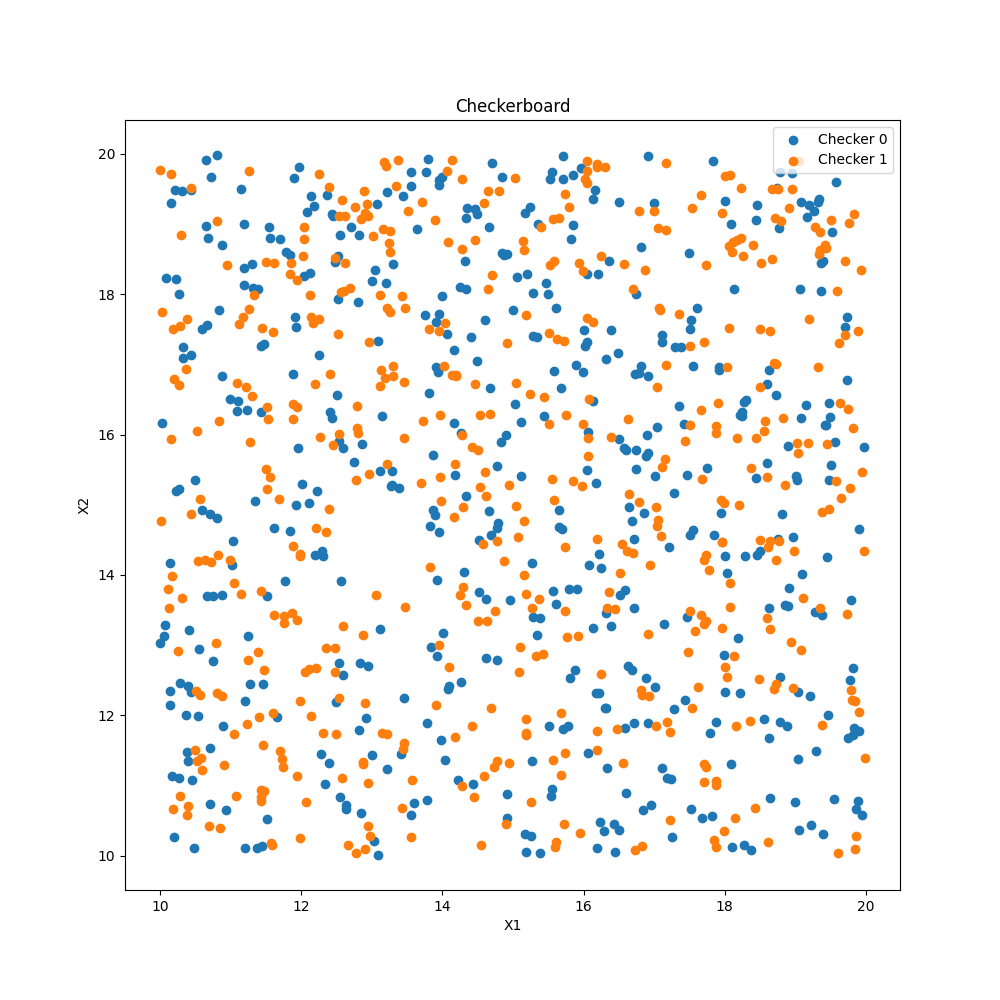
\includegraphics[width=3.5in]{../images/checkerboard-2.png}
\captionsetup{justification=centering}                                                                                                                                   
\caption{Visualization of the dataset of the alternative problem}
\label{fig:checkerboard2}                                                                                                                                                           
\end{figure}
The model, without any surprise, performs much worse: the maximum accuracy is $\sim55\%$, the loss remains quite high and it never converged (Figure \ref{fig:losacc}).
This means that the model correctly classified a sample almost with the same probability of getting head with a coin toss. 

\begin{figure}%
    \centering
    \subfloat[\centering Loss]{{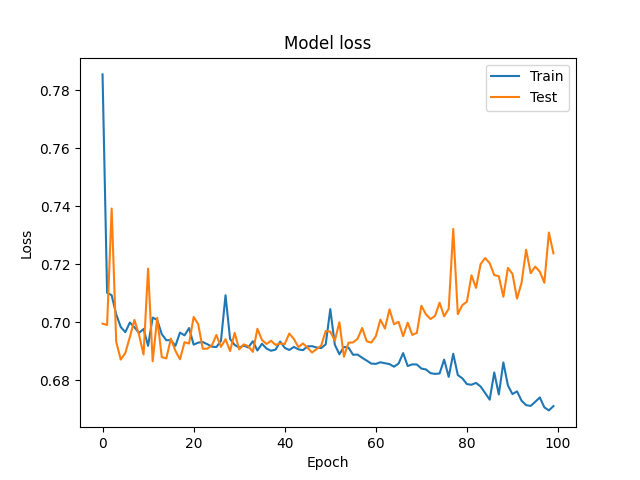
\includegraphics[width=5cm]{../images/loss-1000-20-binary_crossentropy-adam-100-4.png} }}%
    \qquad
    \subfloat[\centering Accuracy]{{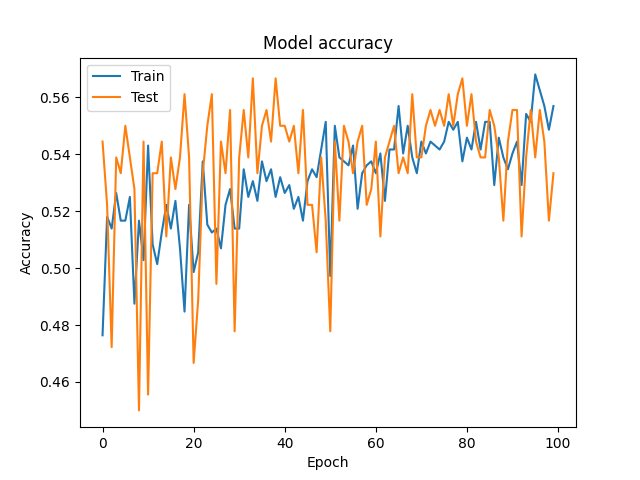
\includegraphics[width=5cm]{../images/accuracy-1000-20-binary_crossentropy-adam-100-4.png} }}%
    \caption{Loss and accuracy plots of the alternative problem}%
    \label{fig:losacc}%
\end{figure}

Figure \ref{fig:decision2} shows how the model could not find any pattern, changing quite frequently its decision boundaries

\begin{figure}[ht!]
\begin{tabular}{cccc}
\subfloat[1 epoch]{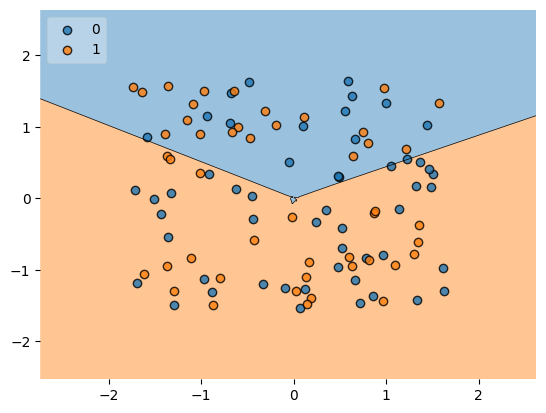
\includegraphics[width = 1in]{../images/regions/0-region-v.png}} &
\subfloat[10 epochs]{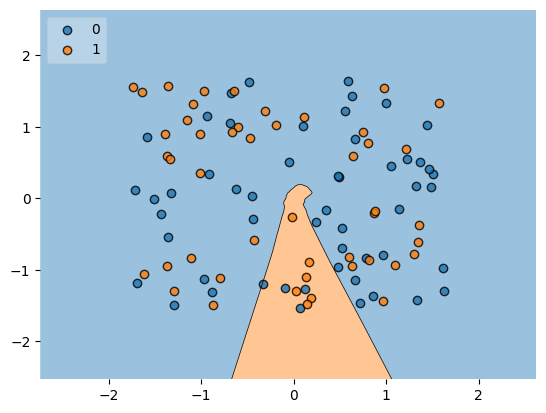
\includegraphics[width = 1in]{../images/regions/10-region-v.png}} &
\subfloat[20 epochs]{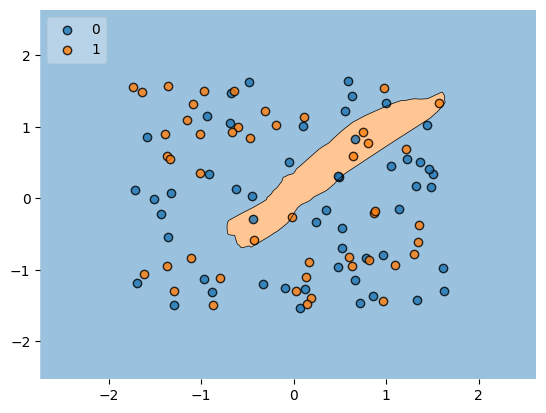
\includegraphics[width = 1in]{../images/regions/20-region-v.png}}\\
\subfloat[30 epochs]{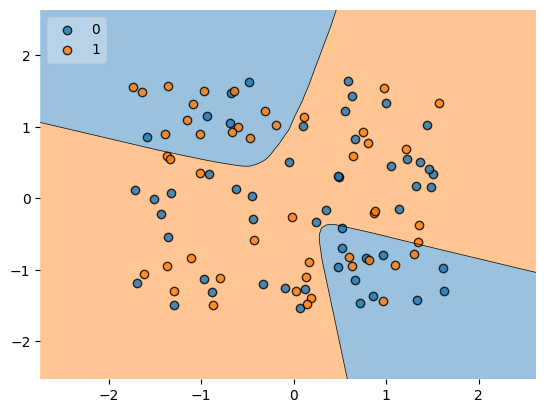
\includegraphics[width = 1in]{../images/regions/30-region-v.png}} &
\subfloat[40 epochs]{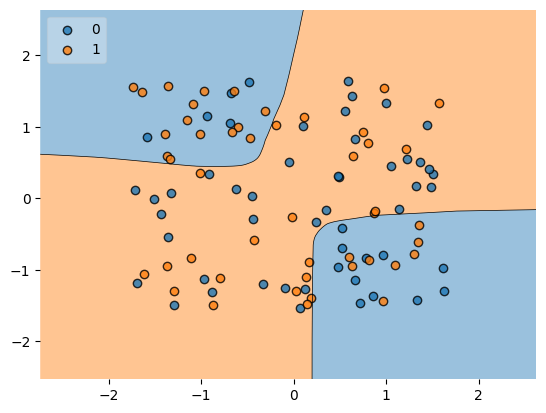
\includegraphics[width = 1in]{../images/regions/40-region-v.png}} &
\subfloat[50 epochs]{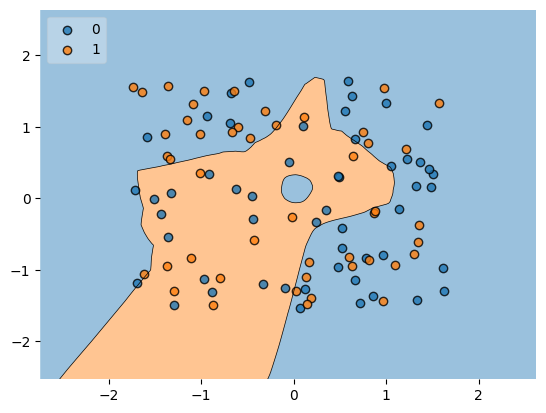
\includegraphics[width = 1in]{../images/regions/50-region-v.png}}\\
\subfloat[60 epochs]{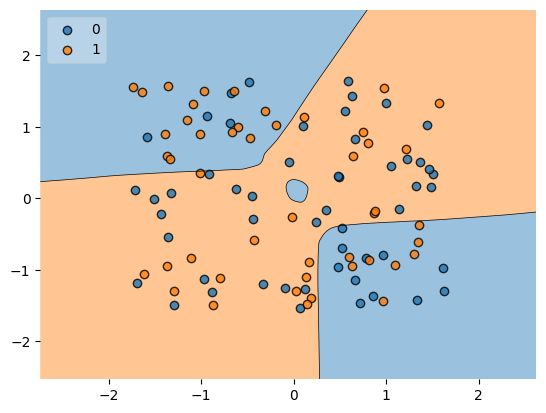
\includegraphics[width = 1in]{../images/regions/60-region-v.png}} &
\subfloat[70 epochs]{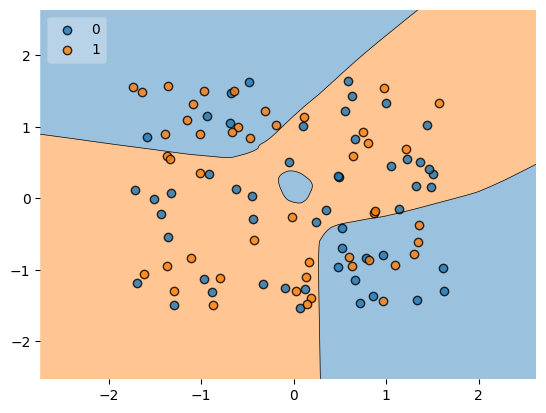
\includegraphics[width = 1in]{../images/regions/70-region-v.png}} &
\subfloat[80 epochs]{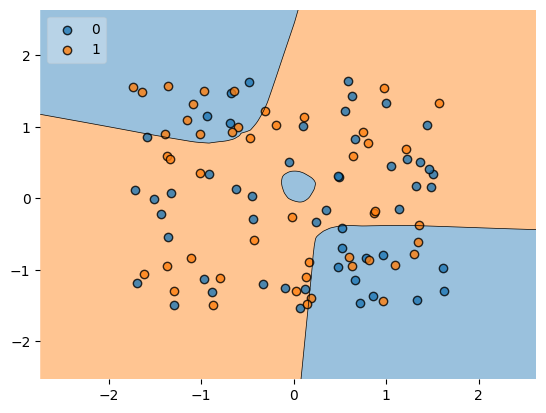
\includegraphics[width = 1in]{../images/regions/80-region-v.png}} 
\end{tabular}
\caption{Evolution of decision boundaries during the training of the alternative problem}
\label{fig:decision2}                                                                                                                                                           
\end{figure}


\section{Other experiments}
In this section we briefly documented the experiments with other optimizers: \emph{SGD} and \emph{RMSprop}. 
Even if their results where good, they converged slower than \emph{Adam}. \par

\emph{RMSprop} converged faster than \emph{SGD} but it had difficulties on escaping local minima, having the loss function over test data to be more swinging (Figure \ref{fig:r1}).


\begin{figure}[ht!]
\centering                                                                        
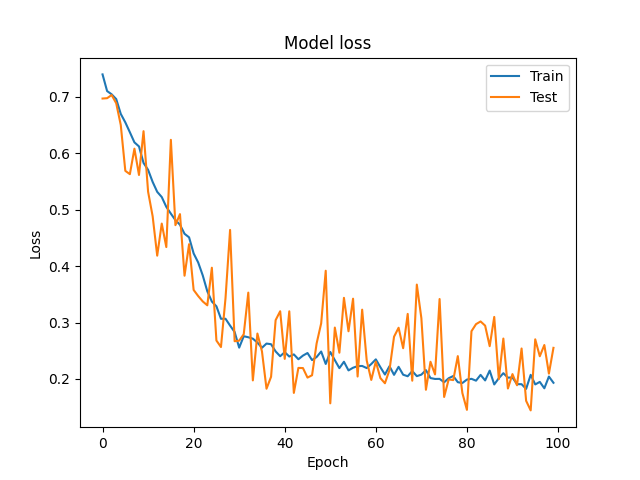
\includegraphics[width=3.5in]{../images/loss-4000-6-binary_crossentropy-rmsprop-100-4.png}
\captionsetup{justification=centering}                                                                                                                                   
\caption{Loss of \emph{RMSprop}}
\label{fig:r1}
\end{figure}

\begin{figure}[ht!]
\centering                                                                        
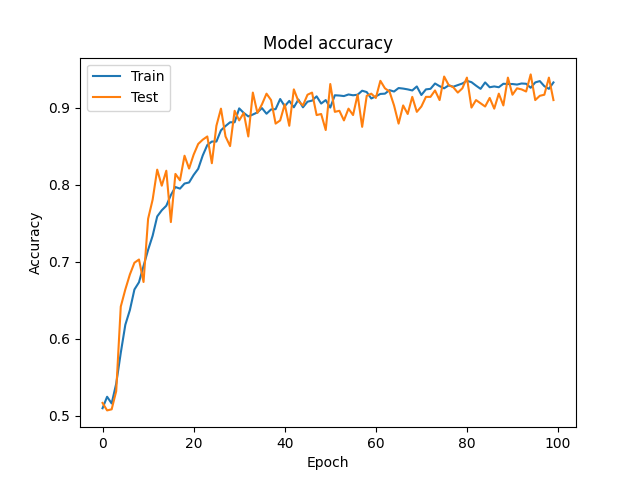
\includegraphics[width=3.5in]{../images/accuracy-4000-6-binary_crossentropy-rmsprop-100-4.png}
\captionsetup{justification=centering}                                                                                                                                   
\caption{Accuracy of \emph{RMSprop}}
\label{fig:r2}
\end{figure}


\emph{SGD} converged slower than \emph{RMSprop} but seemed to be slighty better in escaping local minima regions (Figure \ref{fig:s1}).


\begin{figure}[ht!]
\centering                                                                        
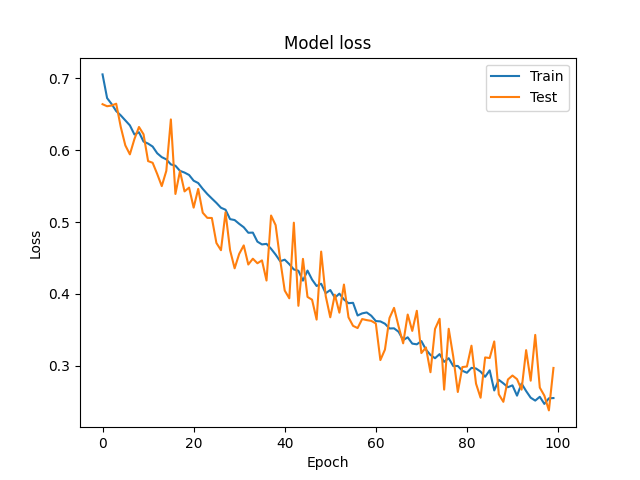
\includegraphics[width=3.5in]{../images/loss-4000-6-binary_crossentropy-sgd-100-4.png}
\captionsetup{justification=centering}                                                                                                                                   
\caption{Loss of \emph{SGD}}
\label{fig:s1}
\end{figure}

\begin{figure}[ht!]
\centering                                                                        
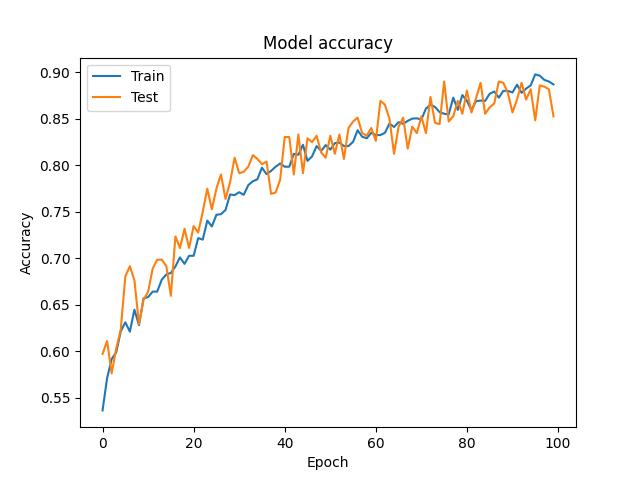
\includegraphics[width=3.5in]{../images/accuracy-4000-6-binary_crossentropy-sgd-100-4.png}
\captionsetup{justification=centering}                                                                                                                                   
\caption{Accuracy of \emph{SGD}}
\label{fig:s2}
\end{figure}

\section{Implementation}
The training can be started with \texttt{assignment1.py}. It generates the needed images for the project in \texttt{./images} and \texttt{./images/regions} along with
a model checkpoint (hdf5 file) in the same script's directory.\par
The validation can be performend with \texttt{evaluation1.py}. It also generates images in \texttt{./images}.\par


\section{Conclusion}
We trained a dense multi-layer Feedforward Neural Network to classify points in a \emph{checker pattern}. We tried many configurations and
a network with 4 dense layers wtih the non-linear activation function \texttt{LeakyReLU} gave goods results and not too long
training times. The chosen optimizer was \emph{Adam} that let the model converge faster and with higher accuracy than the others.
While the goal of the task had been achived reaching an accuracy of $94\%$, the model failed to recognize the pattern itself, overfitting the data; it learned
a cross-like pattern with a checkerboard in the center.


\bibliographystyle{ieeetr}
\bibliography{Bibliography}

\begin{thebibliography}{9}

\bibitem{unlearnable} 
The Unlearnable Checkerboard Pattern
\\Communications of the Blyth Institute Volume 1, Issue 2
\href{https://doi.org/10.33014/issn.2640-5652.1.2.full}{https://doi.org/10.33014/issn.2640-5652.1.2.full}



\end{thebibliography}


\end{document}









